% !TEX root = ../main.tex
% Chapter 3 --- Data
\chapter{Data}\label{ch:data}

In the scope of this work, we use two main data sources. The ERA5 and related datasets provide the coarse-resolution meteorological fields that serve as the model input, while the MeteoSwiss dataset provides the high-resolution measurement data we consider as ground truth for daily maximum temperature and precipitation accumulation. All of them are used over the five years 2020--2024: the models are trained and cross-validated on 2020--2023, and 2024 is held out for the final evaluation (\sref{subsec:meth-cv}). In addition, we use the DHM25 digital elevation model (DEM) to provide the topographical context for the prediction task. The fields used are summarised in \tref{tab:data-grids}. The following sections describe the datasets and the preprocessing steps in more detail.

\begin{table}[htbp]
    \centering
    \caption[Input and target grids]{The two ERA5 input grids~\cite{hersbach2020era5, munozsabater2021era5land} and the MeteoSwiss target grid~\cite{meteoswiss_ogd_grid}.}
    \label{tab:data-grids}
    \footnotesize
    \begin{tabular}{|p{2.2cm}|p{3.5cm}|p{3.5cm}|p{3.5cm}|}
        \hline
        & \textbf{ERA5} & \textbf{ERA5-Land} & \textbf{MeteoSwiss} \\
        \hline
        Product type & Global atmospheric reanalysis: weather model plus observations via data assimilation & Land-surface model rerun forced by ERA5; no data assimilation of its own & Gridded observational analysis, interpolated from the Swiss station network \\
        \hline
        Grid spacing$^{*}$ & $0.25^{\circ} \times 0.25^{\circ}$ (${\sim}19$--$28\,\mathrm{km}$ over Switzerland) & $0.1^{\circ} \times 0.1^{\circ}$ (${\sim}8$--$11\,\mathrm{km}$ over Switzerland) & $1\,\mathrm{km} \times 1\,\mathrm{km}$ on the Swiss LV95 grid.\\
        \hline
        Period / time step & 1940--present, hourly & 1950--present, hourly & TmaxD 1971--, RhiresD 1961--present, daily \\
        \hline
        Fields & Surface and near-surface fields~\cite{era5_single_levels}; upper-air fields on pressure levels~\cite{era5_pressure_levels} & Land and near-surface fields only~\cite{era5land_daily}; no upper-air fields & Daily maximum $2\,\mathrm{m}$ temperature (TmaxD); daily precipitation sum (RhiresD) accumulated from $06\,\mathrm{UTC}$ to $06\,\mathrm{UTC}$\\
        \hline
        Orography handling & Coarse model orography & Daily lapse-rate correction of temperature to the fine-grid elevation; pressure and humidity kept consistent; precipitation inherited from ERA5 & Stations sample the real terrain; interpolation accounts for elevation~\cite{frei2014temperature} \\
        \hline
        Role in this work & Atmospheric input channels: geopotential, temperature, humidity and wind on pressure levels & Surface input channel: daily maximum $2\,\mathrm{m}$ temperature; static geopotential, divided by $g$, for the model orography & Ground truth: training targets and evaluation reference \\
        \hline
    \end{tabular}
    \par\vspace{2pt}
    {\raggedright\scriptsize $^{*}$\,ERA5 and ERA5-Land use regular latitude--longitude grids, so their grid spacing in km varies with latitude.\par}
\end{table}

\section{Meteorological Model Inputs: ERA5}\label{sec:data-era5}

ERA5 is a global meteorological reanalysis product produced by the European Centre for Medium-Range Weather Forecasts (ECMWF)~\cite{hersbach2020era5}. It combines a numerical weather model with observations through data assimilation to give a physically consistent record of the atmosphere. We access it through the Copernicus Climate Data Store (CDS).

ERA5-Land is the land-surface reanalysis derived from ERA5~\cite{munozsabater2021era5land, era5land_daily}. It is produced by running ECMWF's land-surface model on its own, controlled by the near-surface fields of ERA5, on a finer grid. To force the land model on the finer grid, the ERA5 fields are first interpolated horizontally to $0.1^{\circ}$.  The refined surface temperature is then corrected to the true elevation of each fine cell.

Temperature varies with altitude in a well-defined way; this correction recovers part of the mountain and valley structure that the coarse ERA5 grid averages away. This correction applies only to the thermodynamic fields; however, precipitation is taken over from ERA5 as forcing and gains no real sub-grid detail beyond the interpolation to the finer grid.

\section{MeteoSwiss Targets: Temperature and Precipitation}\label{sec:data-targets}

The MeteoSwiss dataset provides the high-resolution measurement data we consider as ground truth for daily maximum temperature and precipitation accumulation. We use the gridded products TmaxD for temperature and RhiresD for precipitation~\cite{meteoswiss_ogd_grid}. Both are derived from the MeteoSwiss station network by spatial interpolation \cite{frei2014temperature,frei1998precip} and are provided on a regular $1\,\mathrm{km} \times 1\,\mathrm{km}$ grid in the Swiss LV95 coordinate system, at a temporal resolution of one day. Note that the $1\,\mathrm{km}$ grid spacing overstates the real information content: the effective resolution is limited by the density of the station network.

The precipitation target is not a calendar-day total. RhiresD accumulates from $06\,\mathrm{UTC}$ to $06\,\mathrm{UTC}$ of the following day, and the value carries the date of the day on which the accumulation begins~\cite{meteoswiss_rhiresd_doc}. The ERA5 input day is the UTC calendar day, so the target day and the input day do not cover the same twenty-four hours; the offset is quantified in \sref{subsec:data-coords}. The two roles ERA5-Land plays are therefore kept strictly apart. As a model \emph{input} channel it enters as the UTC calendar-day total, accumulated $00$--$00\,\mathrm{UTC}$, and the six-hour offset against the target is part of what the model has to work around. As the \emph{evaluation reference} it is re-accumulated over the same $06$--$06\,\mathrm{UTC}$ window as RhiresD, so that reference and target cover the same twenty-four hours and the skill scores of \cref{ch:single-model} compare like with like (\sref{subsec:app-skill-precip}).

\section{Topography (DHM25): DEM and TPI}\label{sec:data-topography}

High-resolution topography for this project has been prepared by the predecessor project of \textcite{passos}; no modifications have been made within this project. The height data is derived from the $25\,\mathrm{m}$ swisstopo DHM25 digital height model (DEM), described by \textcite{swisstopo_dhm25}, and is stored on a regular $50\,\mathrm{m}$ grid in the Swiss LV95 coordinate system. It provides the elevation MLP with the local elevation, the elevation difference to the coarse input grid, and the topographic position index at a $500\,\mathrm{m}$ scale (TPI-500\footnote{The topographic position index compares the elevation of each point with the mean elevation of the surrounding terrain within a given radius, here $500\,\mathrm{m}$: positive values mark ridges and hilltops, negative values valleys, and values near zero flat ground or uniform slopes, following \textcite{weiss2001tpi}.}). The MeteoSwiss target coordinates are given in WGS84, so we transform them to LV95 and bilinearly interpolate the topographic fields at each $1\,\mathrm{km}$ target point.

\section{Preprocessing and Features}\label{sec:data-preprocessing}

\subsection{Coordinate Alignment and Normalisation}\label{subsec:data-coords}
The three datasets have different coordinate systems and grid resolutions, so they need to be aligned and normalised before they can be used together. \textcite{passos} established a workflow to align the MeteoSwiss target points with the ERA5-Land surface field. We keep the core approach, but to provide compatibility with the atmospheric input, some adjustments were necessary and are described below.

One point governs everything that follows: the datasets are never projected onto a single common grid. Two frames coexist by design. The \emph{encoder grid} is a regular latitude--longitude lattice and carries the input channels; the \emph{target points} are the MeteoSwiss locations, handled as an unstructured list of coordinates rather than as a lattice. The only link between them is the squared-distance matrix of step~\ref{item:data-grid-geometry}, which the final layer turns into an interpolation kernel. What is shared is the domain: the ERA5-Land $0.1^{\circ}$ field is loaded first, and its bounding box fixes the latitude and longitude range against which every coordinate in the pipeline, on either side, is normalised.

In practice, every coordinate system gets reprojected onto the shared WGS84 domain above, the encoder grid is picked for whichever configuration is running (the native ERA5-Land or ERA5 lattice), the DHM25 topography is looked up at each target point, and the distance matrix the RBF layer needs is built from there. Each field is then normalised in whatever way fits it: weather channels and the temperature target are $z$-scored, coordinate and seasonal channels are already bounded so they are left as they are, and precipitation stays in raw millimetres so the exact zeros the Bernoulli--Gamma head needs are not shifted away from zero. All of these normalisation numbers are saved with the trained model, so new data is normalised the same way later on. The full step-by-step version, including the exact order of operations and the six-hour offset between the UTC-day input and the precipitation target's accumulation window, is in \sref{sec:app-preprocessing}.

\tref{tab:data-context} lists the composition of each configuration and the stage
at which every input enters the architecture; \fref{fig:input-channels} shows the
surface and atmospheric sets in detail.

\begin{table}[htbp]
    \centering
    \caption[Model inputs and where they enter]{Inputs to the model and the stage at which they enter. The upper block gives the encoder context for the configurations compared in this work, where the scaffold denotes the two coordinate channels, the two seasonal channels and the elevation channel. The lower block gives the remaining inputs, which are the same in every configuration. $P$ is the number of target points and $B$ the number of days in a batch. The pressure-level variables are given by their ERA5 short names: $z$ geopotential, $t$ temperature, $q$ specific humidity, $u$ and $v$ the eastward and northward wind components. The surface field of the ERA5-Land configurations is $\mathrm{t2m\_max}$, the daily maximum $2\,\mathrm{m}$ temperature; the surface precipitation configuration adds $\mathrm{tp}$, the daily precipitation total; the two surface anchors of the atmospheric configuration are $\mathrm{t2m}$, the $2\,\mathrm{m}$ temperature, and $\mathrm{tp}$, the total precipitation. The six levels are $1000$, $925$, $850$, $700$, $500$ and $300\,\mathrm{hPa}$, and the five hours are $00$, $06$, $12$, $15$ and $18$ UTC.}
    \label{tab:data-context}
    \footnotesize
    \begin{tabular}{|p{3.2cm}|p{2.8cm}|p{4.6cm}|p{2.1cm}|}
        \hline
        \textbf{Input} & \textbf{Entry Point} & \textbf{Content} & \textbf{Dimension} \\
        \hline
        \multicolumn{4}{|l|}{\textit{Encoder context: one tensor per day, assembled as described above}} \\
        \hline
        Surface --- baseline & Encoder, ERA5-Land $0.1^{\circ}$ & $\mathrm{t2m\_max}$ + scaffold & 6 channels \\
        \hline
        Surface without elevation$^{*}$ & Encoder, ERA5-Land $0.1^{\circ}$ & $\mathrm{t2m\_max}$ + scaffold without the elevation channel & 5 channels \\
        \hline
        Surface precipitation & Encoder, ERA5-Land $0.1^{\circ}$ & $\mathrm{tp}$ + $\mathrm{t2m\_max}$ + scaffold & 7 channels \\
        \hline
        Atmospheric & Encoder, ERA5 $0.25^{\circ}$ & 3 variables ($z$, $t$, $q$) $\times$ 6 levels $\times$ 5 hours + scaffold & 95 channels \\
        \hline
        Atmospheric with surface anchors & Encoder, ERA5 $0.25^{\circ}$ & 3 variables ($z$, $t$, $q$) $\times$ 6 levels $\times$ 5 hours + $\mathrm{t2m}$ and $\mathrm{tp}$ $\times$ 5 hours + scaffold & 105 channels \\
        \hline
        Atmospheric with wind & Encoder, ERA5 $0.25^{\circ}$ & 5 variables ($z$, $t$, $q$, $u$, $v$) $\times$ 6 levels $\times$ 5 hours + scaffold & 155 channels \\
        \hline
        \multicolumn{4}{|l|}{\textit{Further inputs: identical in every configuration}} \\
        \hline
        Distance matrix & Final layer & Squared distance in degrees from every target point to every point of the input grid & $(P, \mathrm{lat}, \mathrm{lon})$ \\
        \hline
        Topographic features & Elevation MLP & Elevation, difference to the model orography, TPI-500 & $(P, 3)$ \\
        \hline
        Seasonal features & Elevation MLP & $\cos$ and $\sin$ of the day of year, also present as two context channels & $(B, 2)$ \\
        \hline
    \end{tabular}
    \par\vspace{2pt}
    {\raggedright\scriptsize $^{*}$\,These five channels are exactly the encoder context of the predecessor project of \textcite{passos}, which passed the surface temperature, the two coordinates, and the two seasonal channels to the encoder and kept all elevation information in the elevation MLP. Of the configurations studied here, this one is therefore the closest in methodology to that work.\par}
\end{table}

\begin{figure}[H]
    \centering
    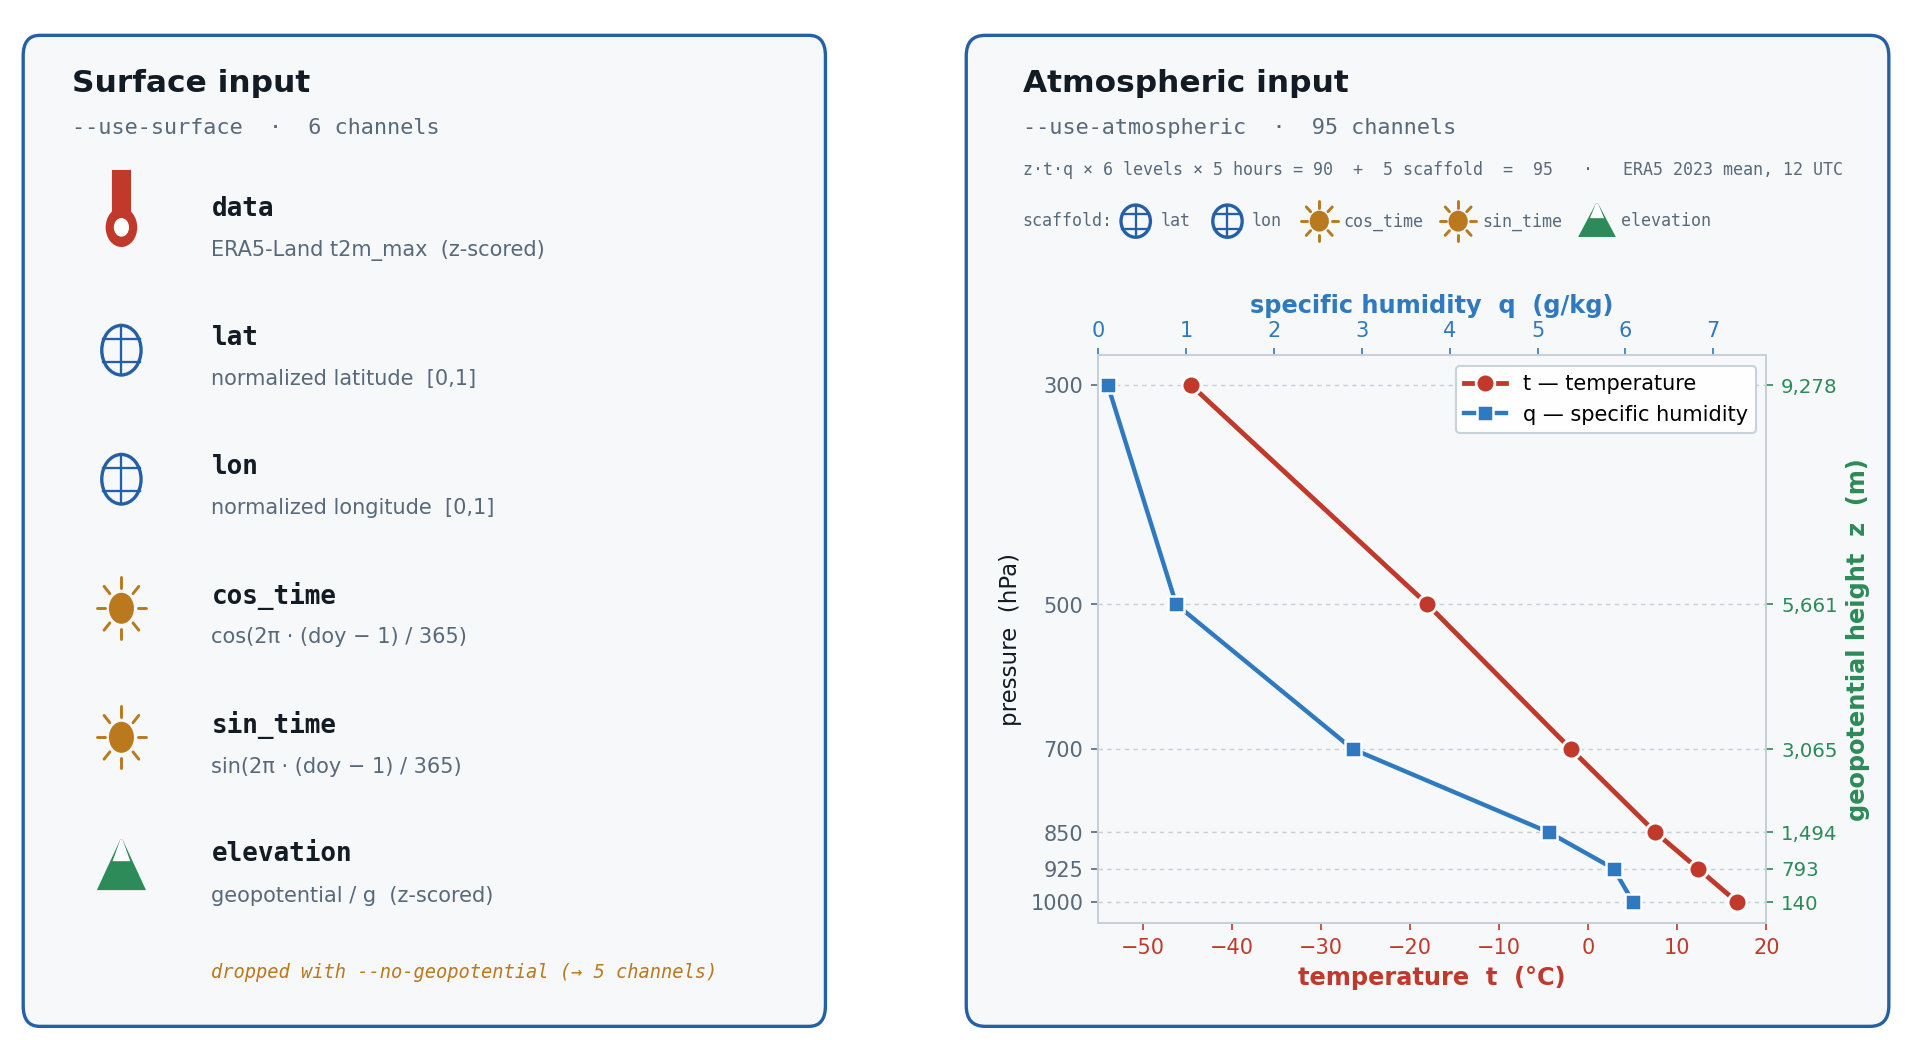
\includegraphics[width=0.9\textwidth]{images/12_input_channels.png}
    \caption[The surface and atmospheric input channel sets]{The two input channel sets of \tref{tab:data-context} in detail. Left: the six surface channels with their normalisation. Right: the atmospheric set, where geopotential, temperature and specific humidity are taken at six pressure levels and five times of day ($90$ channels), plus the same five scaffold channels, giving $95$. Wind components enter only in the extended atmospheric configuration. The emagram marks the six pressure levels on the domain-mean ERA5 profile for 2023 at 12~UTC, with geopotential height on the right-hand axis.}
    \label{fig:input-channels}
\end{figure}

\subsection{Differences to the Predecessor Project}\label{subsec:data-predecessor}

Three points depart from the inherited pipeline.
\begin{itemize}
    \item \textbf{Alignment of the input grid} Every file's coordinates are snapped to five decimals before the yearly ERA5 files are merged, since ERA5 stores the same grid line with a drift of about $10^{-13}$ degrees between files. Five decimals is about a metre on the ground, far finer than the $0.1^{\circ}$ spacing of the grid and far coarser than the drift, so the snap moves no grid cell and the files merge onto one common lattice.
    \item \textbf{Normalisation statistics} The predecessor normalised a single surface field with statistics recomputed from whatever data was being loaded, and stored only those two numbers. In this work, we follow the principle that every channel needs its own statistics, and they must be stored with the model, or a model applied to a new year is normalised differently than it was trained. Within the same rework, we made the target normalisation configurable, so precipitation stays in millimetres while temperature is standardised.
    \item \textbf{Elevation input channel} In the predecessor project, elevation reached the model only through the elevation MLP, never as an input channel to the encoder. This was not a deliberate choice, but a code bug discovered late in the project. Here the geopotential-derived elevation channel is part of the input context unless stated otherwise.
\end{itemize}

Taken together, these differences mean that results obtained with the earlier pipeline are not a suitable baseline for our work. We therefore treat the predecessor project as the starting point of this implementation rather than as a benchmark, and rerun the surface configuration under the corrected pipeline to obtain our own baseline. As an external reference, we use, if applicable, the published results of \textcite{vaughan2022convcnp}, who introduced the downscaling approach we follow here. All comparisons reported below are made against one of these two references (\cref{ch:single-model}).

